\documentclass[11pt]{article}

\usepackage[margin=1in]{geometry}
\usepackage{amsmath,amssymb}
\usepackage{booktabs}
\usepackage{graphicx}
\usepackage{array}
\usepackage{tabularx}
\usepackage{caption}
\usepackage{xcolor}
\usepackage[hidelinks]{hyperref}
\usepackage{microtype}
\usepackage{fontspec}
\usepackage{newtxmath}
\usepackage{titlesec}
\usepackage{titling}

\newcommand{\note}[1]{\texorpdfstring{\textcolor{red}{[NOTE: #1]}}{[NOTE: #1]}}
\newcolumntype{Y}{>{\raggedright\arraybackslash}X}
\defaultfontfeatures{Ligatures=TeX}
\setmainfont{IBM Plex Serif}[
  Path=../../../addenda/typst-field-manual/assets/fonts/,
  UprightFont=IBMPlexSerif-Regular.ttf,
  BoldFont=IBMPlexSerif-Bold.ttf,
  ItalicFont=IBMPlexSerif-Italic.ttf,
]
\setsansfont{IBM Plex Sans Condensed}[
  Path=../../../addenda/typst-field-manual/assets/fonts/,
  UprightFont=IBMPlexSansCondensed-Regular.ttf,
  BoldFont=IBMPlexSansCondensed-Bold.ttf,
]
\setmonofont{IBM Plex Mono}[
  Path=../../../addenda/typst-field-manual/assets/fonts/,
  UprightFont=IBMPlexMono-Regular.ttf,
]
\emergencystretch=2em
\definecolor{specteraccent}{HTML}{1F4555}
\definecolor{spectermuted}{HTML}{616161}

\setlength{\droptitle}{-2.0em}
\pretitle{%
  \begin{flushleft}%
  \color{specteraccent}\rule{\linewidth}{1.2pt}\par
  \vspace{0.85em}%
  {\sffamily\bfseries\small SPECTER LABS PREPRINT\par}%
  \vspace{0.8em}%
  \LARGE\bfseries
}
\posttitle{\par\end{flushleft}\vspace{0.45em}}
\preauthor{\begin{flushleft}\normalsize\sffamily}
\postauthor{\par\end{flushleft}\vspace{0.25em}}
\predate{\begin{flushleft}\small\sffamily\color{spectermuted}}
\postdate{\par\end{flushleft}\vspace{0.95em}}

\titleformat{\section}
  {\normalfont\large\sffamily\bfseries\color{specteraccent}}
  {\thesection.}{0.6em}{}
\titleformat{\subsection}
  {\normalfont\normalsize\sffamily\bfseries}
  {\thesubsection.}{0.6em}{}
\titlespacing*{\section}{0pt}{1.8ex plus .2ex minus .2ex}{0.8ex}
\titlespacing*{\subsection}{0pt}{1.4ex plus .2ex minus .2ex}{0.55ex}
\captionsetup[figure]{font=small,labelfont=bf,textfont=it}
\captionsetup[table]{font=small,labelfont=bf}

\renewenvironment{abstract}{%
  \begin{flushleft}
  \small
  {\sffamily\bfseries Abstract\par}
  \vspace{0.35em}
}{%
  \end{flushleft}
  \vspace{0.65em}
}

\title{Sorting Cells as Morphogenesis, Revisited:\\Mechanisms, Ablations, and Robustness Semantics}
\author{%
  \begin{tabular}{@{}p{0.38\linewidth}@{\hspace{2.5em}}p{0.38\linewidth}@{}}
  Ludwig Pouey & Philip Rhor \\
  {\small\color{spectermuted}Specter Labs} & {\small\color{spectermuted}Specter Labs}
  \end{tabular}
}
\date{February 2026}

\begin{document}
\maketitle

\begin{abstract}
Zhang et al.\ (2024) propose a minimal morphogenesis model in which individual ``cells'' execute
classical sorting rules from a local cell-view state and nonetheless achieve global organization.
In these implementations, however, the operator class is not uniform: Bubble, Insertion,
Gnome, and Shaker use adjacent swaps, whereas 1D Selection performs direct transpositions toward an
ideal position. We revisit the model with a semantics-first analysis that separates action range,
blocked-target policy, and execution substrate.

We report four main results. First, a new $2\times2$ factorization of 1D Selection shows that under
immovable frozen indices only the combination of long-range action and frozen-target rerouting is
robust; adjacent-only variants remain strictly local but fail once barriers are introduced, even
after expending far more work. Second, the rerouting ablation remains decisive within the
published long-range Selection operator class: it yields adaptive Selection success in $270/270$ archived
trials at frozen counts $\{3,6,9\}$ whereas the stubborn variant succeeds in $0/270$. Third, under
matched immovable-index semantics, robustness differences are not attributable to distributed
execution alone: the matched centralized comparison shows exact success/error agreement between
archived cell-view and centralized baselines, while a new matched-substrate comparison shows that
threaded and sequential cell-view schedules also agree on outcomes, with the main substrate effect
appearing in compare-count work rather than in which conditions succeed. Fourth, temporal
separation is positively associated with algotype clustering, and both the \texttt{InsertionNoWait}
ablation and a new transfer experiment
support a timing-based account: exporting the Insertion-style waiting gate to Bubble and Gnome
clones reproduces the predicted rise in temporal separation and clustering.

We retain the 2D section and Directed Flow diagnostic as narrower, secondary results rather than
the paper's main evidential core. By contrast, we frame the K-computation surface as a matched
state-space analysis that is exact for an explicit reachable-state proposal null and conservative
relative to blind operator-walk search. Across the paper, the main lesson is that claims about robustness
or ``basal intelligence'' in sorting-cell systems depend on explicit operator semantics, obstacle
semantics, and matched baselines.
\end{abstract}

\section{Introduction}
\label{sec:intro}
Local-to-global organization is a recurring motif in both developmental biology and distributed
computing. Zhang et al.\ introduce a toy model that intentionally collapses the substrate to its
barest computational ingredients: a 1D line (or 2D grid) of agents that update from a local
cell-view state according to simple rules derived from classical sorting algorithms
\cite{zang2024classical}. Many of those rules use adjacent swaps, but the published 1D Selection
implementation instead performs direct transpositions toward an explicit ideal position.
Despite minimal sensing and communication, the system exhibits:
(i) reliable convergence to an ordered configuration in 1D,
(ii) algotype clustering (cells running the same algorithm become spatially adjacent),
and (iii) robustness to perturbations such as frozen (damaged) cells.

This follow-up has a deliberately narrow scope: we do not propose a new model class.
Instead, we push the original claims by adding targeted measurements and ablations, and by clarifying
semantics that strongly affect conclusions.

\paragraph{Guiding questions.}
We focus on seven questions:
\begin{enumerate}
  \item \textbf{Mechanism:} what is the minimal causal mechanism sufficient to explain algotype
  clustering?
  \item \textbf{Operator classes:} which parts of Selection's robustness come from action range,
  and which come from frozen-target rerouting?
  \item \textbf{Ablation:} within the published Selection operator class, which specific rule is
  responsible for robustness and ``navigation'' in the presence of obstacles?
  \item \textbf{Central claim test:} is the distributed cell-view implementation more robust than a
  centralized baseline when both face identical frozen-index constraints?
  \item \textbf{Dimensionality:} which behaviors generalize to 2D ordering targets, and what fails?
  \item \textbf{Structure in dynamics:} do swap-interaction graphs expose algorithmic signatures that
  align with (or fail to predict) task success?
  \item \textbf{Search efficiency:} can we quantify how much ``smarter'' each algorithm is relative to
  a blind random-walk baseline, using the K-computation framework of Chis-Ciure and Levin
  \cite{chisciure2025cognition}?
\end{enumerate}

\paragraph{Summary of findings.}
Temporal separation between algorithm classes is positively associated with clustering, with the
strongest signal concentrated in Insertion-containing mixtures, and a targeted ablation strongly
supports a timing-based mechanism. Under immovable obstacles, a new factorization experiment shows
that the published 1D Selection behavior depends jointly on long-range transpositions and
frozen-target rerouting. The rerouting ablation then isolates that half of the result within the
original Selection operator class. The centralized and matched-substrate comparisons then show that
distributed execution itself is not the
source of the robustness difference: matched baselines reproduce the same paired outcomes, although
the threaded substrate can require dramatically more work for published Selection. The 2D section
and Directed Flow remain secondary and more limited in scope than the 1D core, and the K section
is presented as a matched exact state-space analysis rather than as a descriptive fixed-baseline
curve.

\section{Model and Metrics}
\label{sec:methods}
\subsection{Sorting cells and operator classes}
We adopt the Zhang et al.\ multithreaded ``cell-view'' implementation: each cell is a thread that
repeatedly decides whether to swap using only bounded local state and shared state protected by a
lock. ``Cell-view'' therefore describes the decision substrate, not a uniform move operator.
Cells are parameterized by an \emph{algotype} (Bubble, Selection, Insertion, etc.), and those
algotypes differ materially in target representation and action range.

\begin{table}[t]
  \centering
  \small
  \begin{tabularx}{\linewidth}{@{}Y Y Y Y@{}}
    \toprule
    Algorithm family & Target representation & Executed move & Blocked-target behavior \\
    \midrule
    Bubble / Insertion / Gnome / Shaker (1D) & Local neighbor comparisons; Insertion also tracks a sorted-prefix gate & Adjacent swap & No rerouting beyond the local rule \\
    Selection (published 1D) & Explicit ideal index in the 1D total order & Direct transposition to the ideal index & Reroute when the desired target index is frozen, or remain stubborn in the ablation \\
    Adjacent Selection & Same explicit ideal index as 1D Selection & One adjacent step toward the ideal index & Same rerouting / stubborn split as above \\
    Selection2D & Explicit ideal position induced by the target order & Neighbor-local greedy grid swap & No long-range transposition; progress is routed through adjacent moves \\
    \bottomrule
  \end{tabularx}
  \caption{Operator classes discussed in this paper. The key distinction is between local
  perception and action range: published 1D Selection has local cell-view execution but a nonlocal
  move operator.}
  \label{tab:operator-classes}
\end{table}

\subsection{Obstacle semantics}
The original paper discusses both movable and immovable damage. In the published code, the term
``frozen cell'' is therefore overloaded; two distinct semantics matter:
\begin{itemize}
  \item \textbf{Movable frozen cells:} frozen cells do not initiate swaps, but can be displaced by
  other cells swapping with them (a ``movable obstacle'').
  \item \textbf{Immovable frozen indices:} certain array indices cannot participate in swaps at all
  (an ``immovable obstacle'' / hard barrier).
\end{itemize}
We use the terms \emph{movable} and \emph{immovable} throughout; each result section states the
semantics explicitly. A compact per-experiment semantics summary and command index are collected in
Appendix~\ref{sec:appendix-repro} so the main text can stay focused on the argument.

\subsection{Clustering}
For a 1D array of length $n$ with algotypes assigned to positions, define instantaneous clustering
as the fraction of adjacent pairs that share the same algotype.
Let $p_t$ be the fraction of cells of type $t$; under random mixing, the baseline adjacent-match
probability is $\sum_t p_t^2$. We report \emph{clustering increase} as:
\[
\Delta C \;=\; \max_{\text{time}} C(t) \;-\; \sum_t p_t^2.
\]

\subsection{Temporal separation}
We define an algorithm's \emph{normalized mean move time} as the average time index (normalized to
$[0,1]$ over the swap sequence) at which cells of that type participate in swaps. For a pair
$(a,b)$, temporal separation is:
\[
S(a,b) \;=\; \left|\mu_a - \mu_b\right|.
\]

\subsection{Dips (``delayed gratification'')}
We operationalize a ``dip'' as a transient increase in a global error metric (1D monotonicity errors
or 2D inversion count) that subsequently recovers to at most the starting value. We use the same dip
detection logic across 1D and 2D trajectories.

\section{Results}
\label{sec:results}

\subsection{Temporal separation predicts clustering}
Figure~\ref{fig:temporal-clustering} shows a positive association between temporal separation and
clustering across the ten pairwise mixtures of five algotypes (Bubble, Selection, Insertion,
Gnome, Shaker). The strongest signal comes from Insertion-containing combinations; non-Insertion
pairs cluster much more weakly. We therefore interpret temporal separation as a major contributor to
clustering, especially for Insertion mixtures, rather than as a universal complete explanation.
The later transfer experiment strengthens that claim by showing that the same timing logic can be transferred to
other local algorithms under same-family controls.

The proposed mechanism is temporal. Selection cells tend to finish early and become quiescent,
whereas Insertion cells activate late because their sorted-prefix gate delays participation until
the left portion of the array is already ordered. This timing mismatch produces temporally
correlated swap bursts where only one algorithm class is still exchanging positions. Cells that move
during the same burst are then more likely to end up adjacent simply because they are the only
cells still rearranging.
The effect is analogous to heterochrony in developmental biology, where shifts in the relative
timing of developmental processes generate spatial structure without explicit coordination or
type-recognition signals.

\begin{figure}[t]
  \centering
  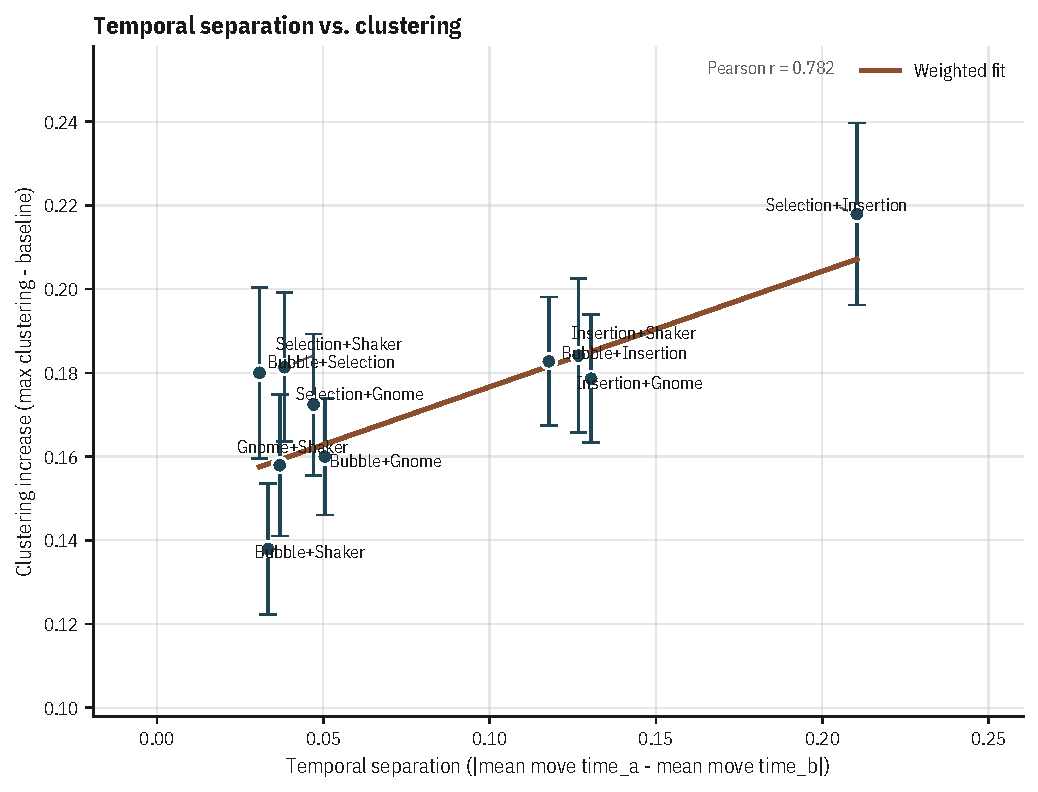
\includegraphics[width=0.85\linewidth]{figures/fig1_temporal_vs_clustering.pdf}
  \caption{\textbf{Temporal separation predicts clustering.}
  Each point is an algorithm pair; $x$ is temporal separation computed from per-algotype normalized
  mean move times; $y$ is clustering increase $\Delta C$ (max clustering minus baseline).
  Error bars show 95\% confidence intervals ($\text{mean} \pm 1.96 \cdot \sigma / \sqrt{n}$,
  $n=50$ trials per pair, $30$ cells).}
  \label{fig:temporal-clustering}
\end{figure}

\subsection{Ablation: removing Insertion's waiting collapses clustering}
If temporal separation is the cause of clustering, then removing the waiting mechanism that makes
Insertion ``late'' should reduce clustering. We implement \texttt{InsertionNoWait} by removing the
enable-to-move gating check, making Insertion behave like other local algorithms (move early).
Figure~\ref{fig:clustering-ablation} shows the expected collapse in clustering, alongside the shift
in the type-2 timing statistic.
This is strong mechanistic evidence for a timing-based account, but we stop short of treating it as
exhaustive causal proof. Seeded per-trial rows are available, but the intervention still
targets one manipulated pair and one weak-clustering control, so the safest claim is that removing
the waiting gate sharply reduces clustering and moves the Bubble+Insertion pair toward a
weak-clustering control.

\begin{figure}[t]
  \centering
  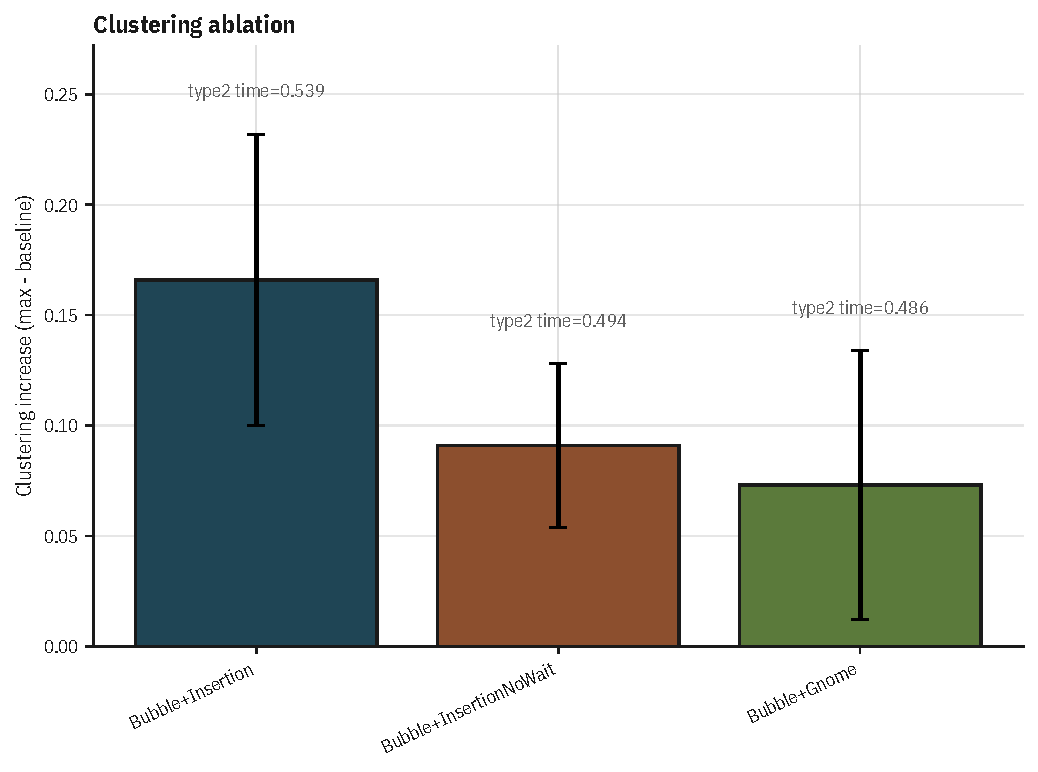
\includegraphics[width=0.85\linewidth]{figures/fig2_clustering_ablation.pdf}
  \caption{\textbf{Clustering ablation.}
  Bubble+Insertion clusters strongly; Bubble+InsertionNoWait clusters weakly and resembles a
  non-separated control (Bubble+Gnome). Annotated values show the mean move time for the second
  algotype, consistent with the proposed timing-to-clustering mechanism.
  Summary statistics are computed over $20$ trials with $50$ cells.
  Error bars indicate $\pm 1$ standard deviation.}
  \label{fig:clustering-ablation}
\end{figure}

\subsection{Synthetic waiting gates transfer clustering beyond Insertion}
If the timing account is broader than native Insertion dynamics, then exporting the same
sorted-prefix waiting gate to another local algorithm should increase temporal separation and
clustering even when operator family is held fixed. We test this by pairing each base
algorithm with a labeled no-delay clone and with a delayed clone that preserves the same local swap
rule but adds the Insertion-style waiting gate.

Across $30$ aggregated trials per pair ($3$ seeds $\times$ $10$ trials, $50$ cells),
Bubble+DelayedBubble yields $\Delta C = 0.176$ and temporal separation $0.111$, compared with the
matched no-delay control Bubble+BubbleClone at $\Delta C = 0.155$ and separation $0.027$.
Gnome+DelayedGnome yields $\Delta C = 0.167$ and separation $0.106$, compared with
Gnome+GnomeClone at $\Delta C = 0.126$ and separation $0.043$. Both delayed-clone pairs move into
the same high-separation regime as Bubble+Insertion ($\Delta C = 0.170$, separation $0.105$),
whereas Bubble+InsertionNoWait remains low ($\Delta C = 0.134$, separation $0.033$).

This materially closes the mechanistic gap left by the original clustering analysis. The waiting
gate is not just an Insertion-specific quirk: when the same timing intervention is transferred to
other local algorithms, clustering rises in the predicted direction under matched same-family
controls. We still avoid the strongest possible universality claim, but the timing account now
generalizes beyond one native algotype.

\begin{figure}[t]
  \centering
  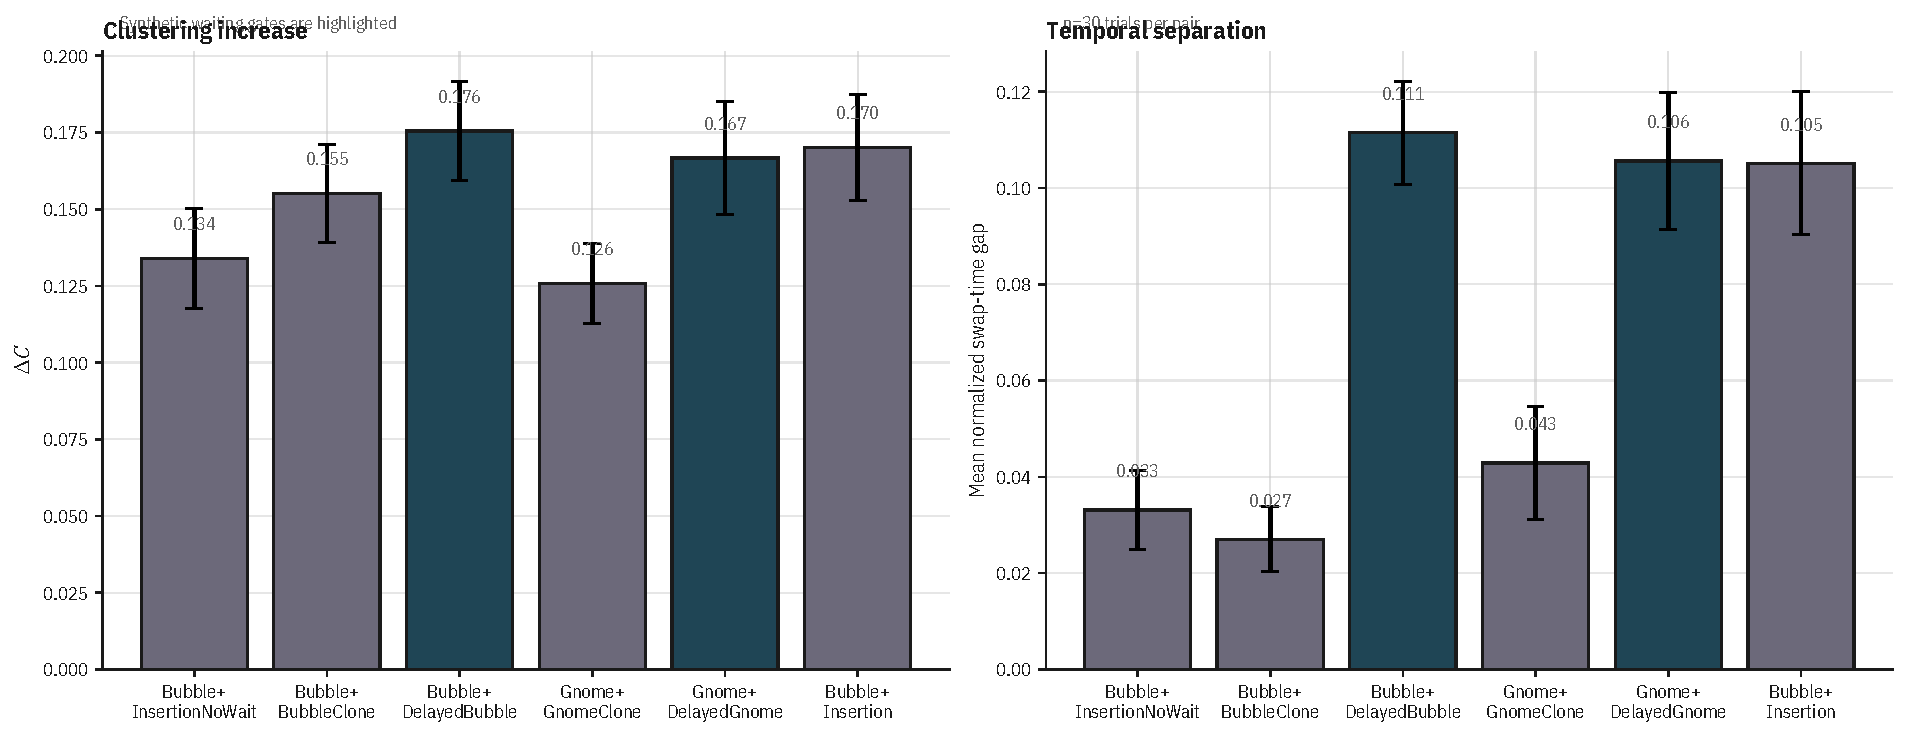
\includegraphics[width=\linewidth]{figures/fig9_timing_interventions.pdf}
  \caption{\textbf{Synthetic waiting gates transfer clustering beyond Insertion.}
  Left: clustering increase $\Delta C$ with 95\% confidence intervals. Right: temporal separation
  with 95\% confidence intervals. Same-family clone controls without the waiting gate stay in the
  low-separation regime, whereas delayed Bubble and delayed Gnome clones move toward the
  Bubble+Insertion reference condition.}
  \label{fig:timing-transfer}
\end{figure}

\subsection{Selection factorization under matched obstacle semantics}
The factorization experiment decomposes Selection robustness into two axes:
(i) action range (direct transposition vs.\ adjacent step) and
(ii) blocked-target behavior (rerouting vs.\ stubbornness).
All four variants share the same 1D ideal-position target representation; only the executed move and
blocked-target policy change.

The immovable panel uses $n=30$, timeout $5$s, seeds $\{40,41,42\}$, and $10$ paired trials per
condition (30 trials total). The movable control uses the same seeds with $5$ paired trials per
condition (15 trials total), tying the factorization back to the original paper's damaged-cell
semantics.

Figure~\ref{fig:exp25} and Table~\ref{tab:exp25} show a clean decomposition under immovable
barriers: only the
long-range+routing quadrant succeeds once frozen indices are introduced. Long-range+stubborn fails
immediately when barriers appear, showing that rerouting is necessary within the published operator
class. Adjacent+routing also fails immediately, showing that rerouting alone is not sufficient when
action range is restricted to adjacent steps. The adjacent variants remain genuinely local in every
condition (weighted mean swap span $= 1.00$), but they fail after expending far more work. At
frozen$=3$, adjacent+routing averages $14{,}917$ swaps and adjacent+stubborn averages $8{,}238$,
versus $91$ for long-range+routing. Under the smaller movable control, long-range+routing retains
limited success at one frozen cell ($3/15$), while the other three variants are $0/15$ as soon as
any frozen cells are introduced.

The main implication is that published 1D Selection's robustness is a joint property of operator
reach and blocked-target adaptation. Published 1D Selection should therefore not be treated as just
another local adjacent-swap rule.

\begin{table}[t]
  \centering
  \small
  \begin{tabular}{@{}lrrrr@{}}
    \toprule
    Variant & Frozen=0 & 3 & 6 & 9 \\
    \midrule
    Long-range + rerouting & 30/30 & 30/30 & 30/30 & 30/30 \\
    Long-range + stubborn & 30/30 & 0/30 & 0/30 & 0/30 \\
    Adjacent + rerouting & 30/30 & 0/30 & 0/30 & 0/30 \\
    Adjacent + stubborn & 30/30 & 0/30 & 0/30 & 0/30 \\
    \bottomrule
  \end{tabular}
  \caption{\textbf{Selection factorization under immovable semantics.}
  Success counts across the $2\times2$ factorization of action range and blocked-target policy.
  Each condition aggregates $30$ paired trials ($3$ seeds $\times$ $10$ trials). Only the
  published long-range+routing combination remains robust once immovable frozen indices are
  introduced.}
  \label{tab:exp25}
\end{table}

\begin{figure}[t]
  \centering
  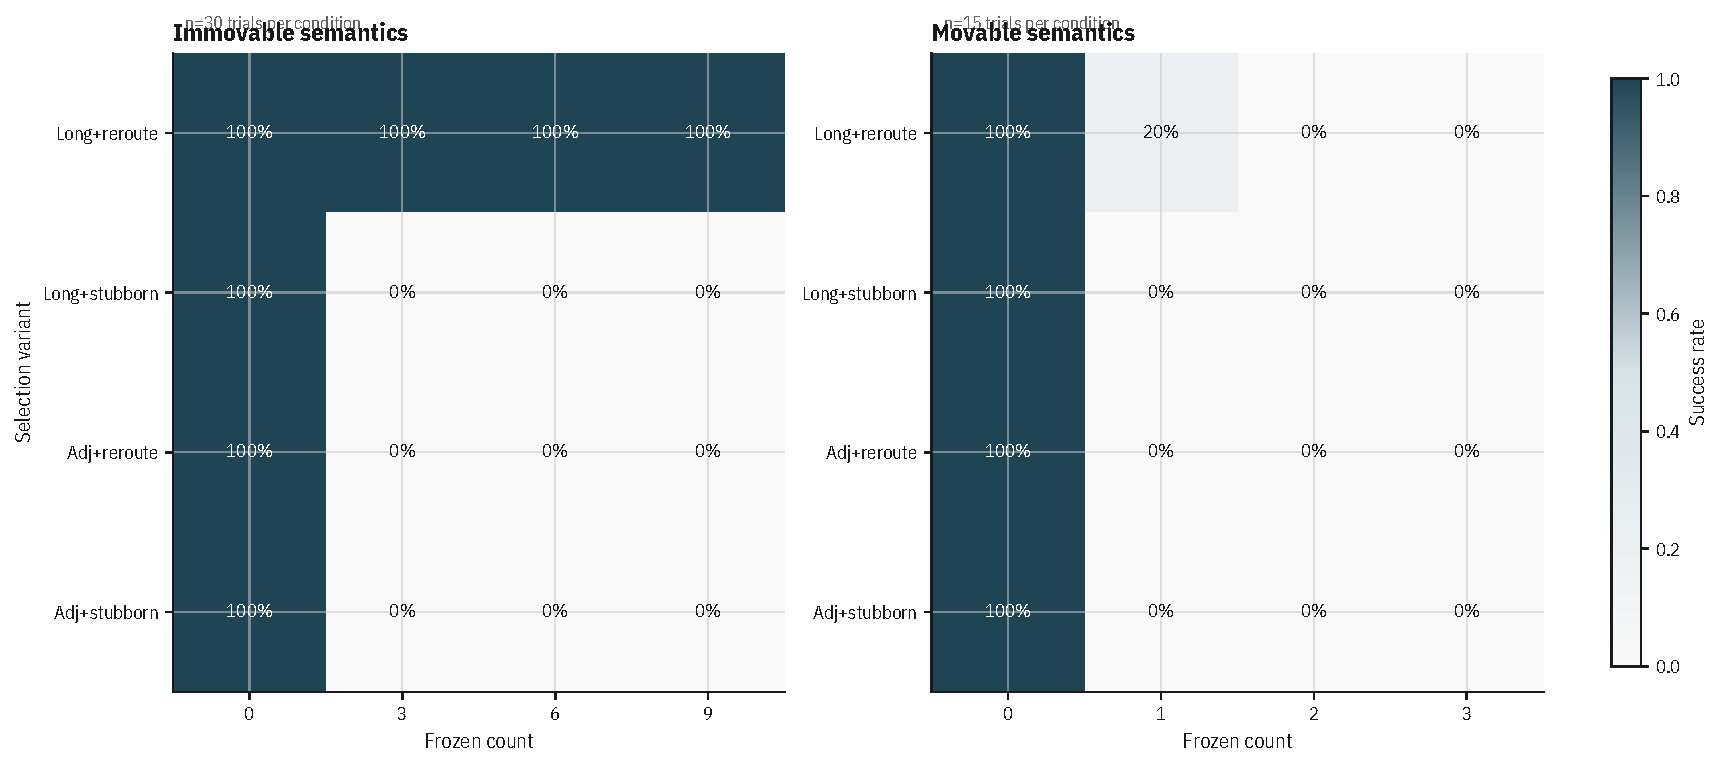
\includegraphics[width=\linewidth]{figures/fig7_selection_factorization.pdf}
  \caption{\textbf{Selection factorization across obstacle semantics.}
  Left: immovable frozen indices. Right: movable frozen cells. Under immovable barriers, only the
  published long-range+routing variant remains successful once obstacles are introduced. Under the
  original movable-damage regime, even that quadrant degrades quickly, showing that obstacle
  semantics materially change the robustness story.}
  \label{fig:exp25}
\end{figure}

\subsection{Frozen-target rerouting within the published Selection operator class}
The factorization result shows that both action range and rerouting matter. The rerouting ablation remains useful because it isolates
the rerouting half of that story within the original long-range Selection operator class.
The ablation is narrower than the phrase ``goal adjustment'' suggests:
\texttt{StubbornSelectionCell} keeps the same direct-target transposition operator and still updates
its active target in some cases, but it removes the specific reroute that occurs when the desired
target index is frozen.

We ran the rerouting ablation with $n=30$ cells, $30$ trials per condition, timeout $10$s, and immovable
frozen-index semantics, aggregated across seeds $\{40,41,42\}$ (90 trials per frozen-count
condition). Within the published long-range Selection operator class, frozen-target rerouting
provides a large and seed-stable benefit: across frozen counts $\{3,6,9\}$, adaptive Selection
achieves $270/270$ success versus $0/270$ for the stubborn ablation.

\begin{table}[t]
  \centering
  \small
  \begin{tabular}{@{}lrr@{}}
    \toprule
    Frozen & Adaptive Selection & Stubborn Selection \\
    \midrule
    0 & 90/90 & 90/90 \\
    3 & 90/90 & 0/90 \\
    6 & 90/90 & 0/90 \\
    9 & 90/90 & 0/90 \\
    \bottomrule
  \end{tabular}
  \caption{\textbf{Frozen-target rerouting ablation, 3-seed aggregate.}
  Success counts under immovable frozen indices. Each condition aggregates $90$ trials
  ($3$ seeds $\times$ $30$ trials). Read together with the factorization result, this supports a narrower and
  stronger claim: rerouting is necessary for robustness \emph{within} the published long-range
  Selection operator class.}
  \label{tab:exp10}
\end{table}

\subsection{Cell-view vs.\ centralized robustness under matched frozen-index semantics}
The original paper motivates cell-view sorting partly through robustness and ``basal intelligence''
arguments. After the factorization and rerouting results, the central remaining question is whether the
\emph{distributed implementation} itself confers robustness beyond the underlying policy and
operator semantics.

The matched centralized comparison evaluates:
(i) traditional centralized Python implementations of Bubble, Insertion, and Selection, and
(ii) the multithreaded cell-view implementations,
under \emph{identical frozen-index constraints} where frozen indices are immovable (cannot participate
in swaps). We paired initial permutations and frozen index sets across implementations.
The traditional baselines were modified to enforce the same frozen-index constraint, rather than
using unmodified textbook code.

With $n=30$ cells, $12$ trials, timeout $10$s, and seeds $\{40,41,42\}$ (36 trials per condition),
we find \textbf{no measurable advantage} of cell-view over centralized baselines in this regime:
for all three algorithms and all tested frozen counts, archived success rates and mean error match
exactly in every seed-condition pair.
Bubble fails once any immovable barrier is present (8.3\% at one frozen index, then 0\%);
Insertion retains limited success at one frozen index (11.1\%), then fails at higher frozen counts;
Selection succeeds at all tested frozen counts.

\begin{table}[t]
  \centering
  \small
  \setlength{\tabcolsep}{4pt}
  \begin{tabular}{@{}lrrrrr@{}}
    \toprule
    Algorithm & Frozen=0 & 1 & 3 & 6 & 9 \\
    \midrule
    Bubble & 36/36 & 3/36 & 0/36 & 0/36 & 0/36 \\
    Insertion & 36/36 & 4/36 & 0/36 & 0/36 & 0/36 \\
    Selection & 36/36 & 36/36 & 36/36 & 36/36 & 36/36 \\
    \bottomrule
  \end{tabular}
  \caption{\textbf{Cell-view vs.\ traditional baseline, 3-seed aggregate.}
  Success counts out of $36$, pooled across seeds $\{40,41,42\}$ ($3$ seeds $\times$ $12$ trials).
  The counts shown are identical for cell-view and traditional implementations in every archived
  seed-condition aggregate.
  Without variance between the cohorts, empirical confidence intervals are degenerate.
  The small per-condition sample ($n=36$) limits power to detect small effects;
  a difference smaller than ${\sim}8\%$ (one-sided 95\% boundary for $0/36$ vs.\ $0/36$)
  cannot be ruled out. In this setting, robustness is dominated by the algorithmic
  rule and obstacle semantics; distributed cell-view execution does not outperform a centralized
  baseline. The archive here is seed-condition aggregate only; the matched-substrate analysis below provides the deeper
  trial-level audit by holding the cell policy fixed and changing only the execution substrate.}
  \label{tab:exp14}
\end{table}

\subsection{Matched cell-view substrates isolate work cost rather than robustness}
The matched centralized comparison above compares cell-view implementations to textbook centralized algorithms, but its archive stores
seed-condition aggregates rather than paired trial rows, and the comparison still changes
both substrate and implementation style. The matched-substrate analysis isolates the substrate question more narrowly by
running the same cell policies under two execution modes:
(i) the original multithreaded cell-view substrate and
(ii) a single-thread scheduler that steps the same cell objects with the same obstacle semantics.
We use a matched compare-and-swap budget of $200{,}000$ and treat textbook centralized algorithms as
a reference surface rather than as part of the matched substrate claim.

In the original-trio panel (Bubble, Insertion, Selection; frozen counts $\{1,3\}$; seeds
$\{40,41,42\}$; $9$ paired trials per condition), threaded, sequential, and textbook runs agree
perfectly on both success and final error in every paired trial. Bubble and Insertion show only
modest threaded/sequential work differences under this metric: the average compare-count ratios are
$1.18\times$ and $1.00\times$ for Bubble at frozen $1$ and $3$, and $1.04\times$ and
$1.11\times$ for Insertion. Published Selection behaves differently: outcomes still match exactly,
but threaded execution consumes far more compare-and-swap events. At frozen $1$, threaded Selection
averages $20{,}116$ compare-and-swap events versus $561$ for the sequential scheduler; at frozen
$3$, the gap is $58{,}423$ versus $597$. These are $35.9\times$ and $97.8\times$ work ratios,
respectively, despite identical paired outcomes. Figure~\ref{fig:exp26} visualizes both the
original-trio work-ratio comparison and the broader Selection-family workload split.

We then extend the same matched-substrate comparison to the broader Selection family
(Selection, StubbornSelection, AdjacentSelection, AdjacentStubbornSelection) across frozen counts
$\{0,1,3,6,9\}$. Across all $45$ paired trials per variant, threaded and sequential substrates
agree on success in every case. For published Selection, paired error also matches perfectly at
every frozen count. The failing variants still agree on success/failure everywhere, but residual
error values diverge more often, indicating that the substrate changes the path through the failure
basin without changing which quadrant succeeds.

Taken together, the centralized and matched-substrate comparisons show that distributed execution is
not what makes the robust conditions robust. In the tested 1D regimes, substrate mainly affects
futile local work before the same outcome is reached.

\begin{table}[t]
  \centering
  \small
  \begin{tabular}{@{}lrrr@{}}
    \toprule
    Algorithm & Frozen=1 ratio & Frozen=3 ratio & Paired outcome match \\
    \midrule
    Bubble & $1.18\times$ & $1.00\times$ & $9/9$ \\
    Insertion & $1.04\times$ & $1.11\times$ & $9/9$ \\
    Selection & $35.86\times$ & $97.84\times$ & $9/9$ \\
    \bottomrule
  \end{tabular}
  \caption{\textbf{Original-trio work ratios (threaded / sequential).}
  Each cell reports the ratio of mean compare-and-swap counts under the matched-substrate pilot
  (3 seeds $\times$ 3 paired trials). Bubble and Insertion show near-parity, whereas published
  Selection incurs far larger substrate-dependent work costs despite perfect paired agreement on
  success and final error.}
  \label{tab:exp26}
\end{table}

\begin{figure}[t]
  \centering
  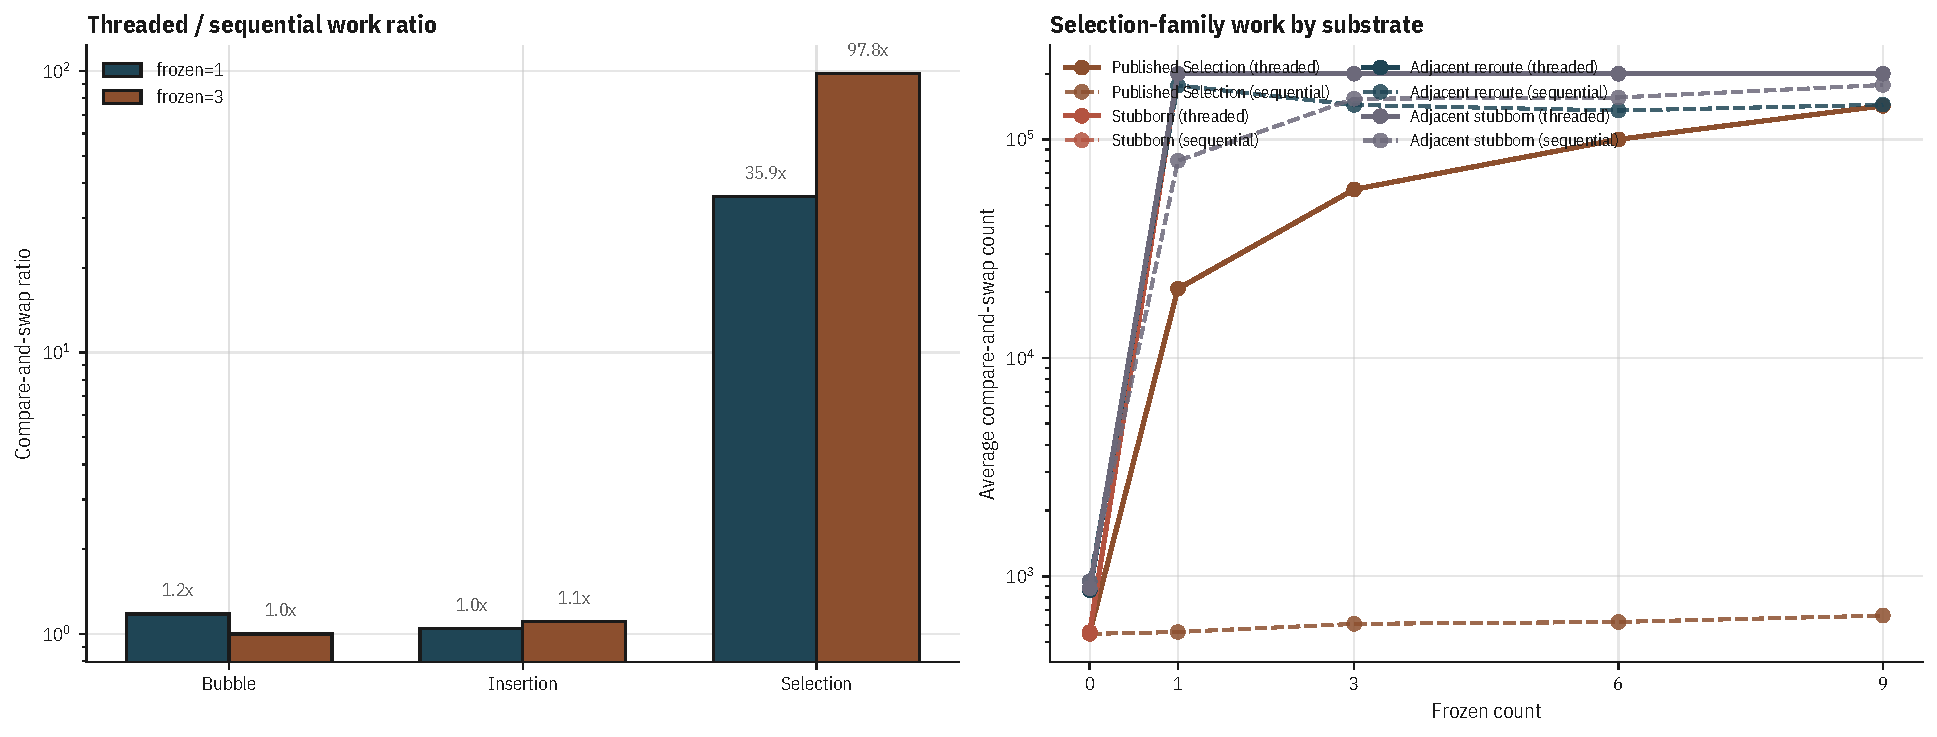
\includegraphics[width=\linewidth]{figures/fig8_substrate_work.pdf}
  \caption{\textbf{Substrate effects appear mainly in compare-count work, not which conditions succeed.}
  Left: threaded/sequential compare-count ratios for the original trio under frozen counts $1$ and
  $3$. Right: Selection-family compare counts by substrate across frozen counts. Published
  Selection shows the strongest substrate-dependent work inflation, whereas Bubble and Insertion
  remain near parity and the failing Selection variants continue to fail under either substrate.}
  \label{fig:exp26}
\end{figure}

\subsection{2D ordering boundary under shell targets}
The move from 1D to 2D is not merely a quantitative scaling but a qualitative change in the
structure of the problem. In 1D, any inversion can eventually be resolved by a sequence of adjacent
swaps: every pair of elements that need to exchange relative order will, at some point, become
neighbors. In 2D with a non-trivial target order such as shell distance, two values that must
exchange relative order may be separated by cells that cannot be permuted by local swaps
alone. This creates non-adjacent inversions that require multi-step routing through the grid, acting
as the 2D analogue of the combinatorial barrier that makes frozen cells fatal for Bubble in 1D,
except that in 2D the barrier exists even without frozen cells.

This section regenerates from a single canonical raw-trial archive (Appendix~\ref{sec:appendix-repro})
and derives the Figure~3 summaries from that source.
We still treat the 2D evidence as narrower than the 1D core because it covers a small
set of operator/target combinations, but its provenance is now explicit and reproducible.

Under the shell-based target order (value increases with squared distance from origin),
we observe a clear boundary:
Bubble2D fails to solve the task, while Selection2D succeeds in the obstacle-free case and then
collapses under immovable frozen cells, with only one small nonzero condition
($4\%$ success on the $6{\times}6$, 8-neighbor, 3-frozen condition).
Figure~\ref{fig:2d-heatmaps} summarizes success rates across grid sizes and neighborhood connectivities.

\paragraph{Alternative ordering targets.}
To confirm that this boundary is not an artifact of the shell-distance target, the canonical 2D
pipeline also evaluates row-major and serpentine (boustrophedon) ordering targets.
Under row-major ordering, the local algorithm (LocalOrder2D) achieves $0\%$ success even without
frozen cells, because row-major introduces non-adjacent inversions that purely local swaps cannot
resolve. Under serpentine ordering (which preserves locality along the space-filling path), the
local algorithm achieves $100\%$ at zero frozen cells but its performance collapses once frozen
cells are introduced, with only one small nonzero condition in the canonical archive
($6\%$ success on the $6{\times}6$, 8-neighbor, 3-frozen setting). SelectionOrder2D achieves
$100\%$ at zero frozen cells across all orderings and connectivities, but also collapses under
frozen cells, retaining only sparse nonzero success in a few $6{\times}6$ conditions.
These controls qualify rather than erase the shell-order boundary: target-order choice can rescue a
purely local algorithm in the zero-obstacle case (serpentine), but not under row-major ordering or
once frozen cells are introduced.

\begin{figure}[t]
  \centering
  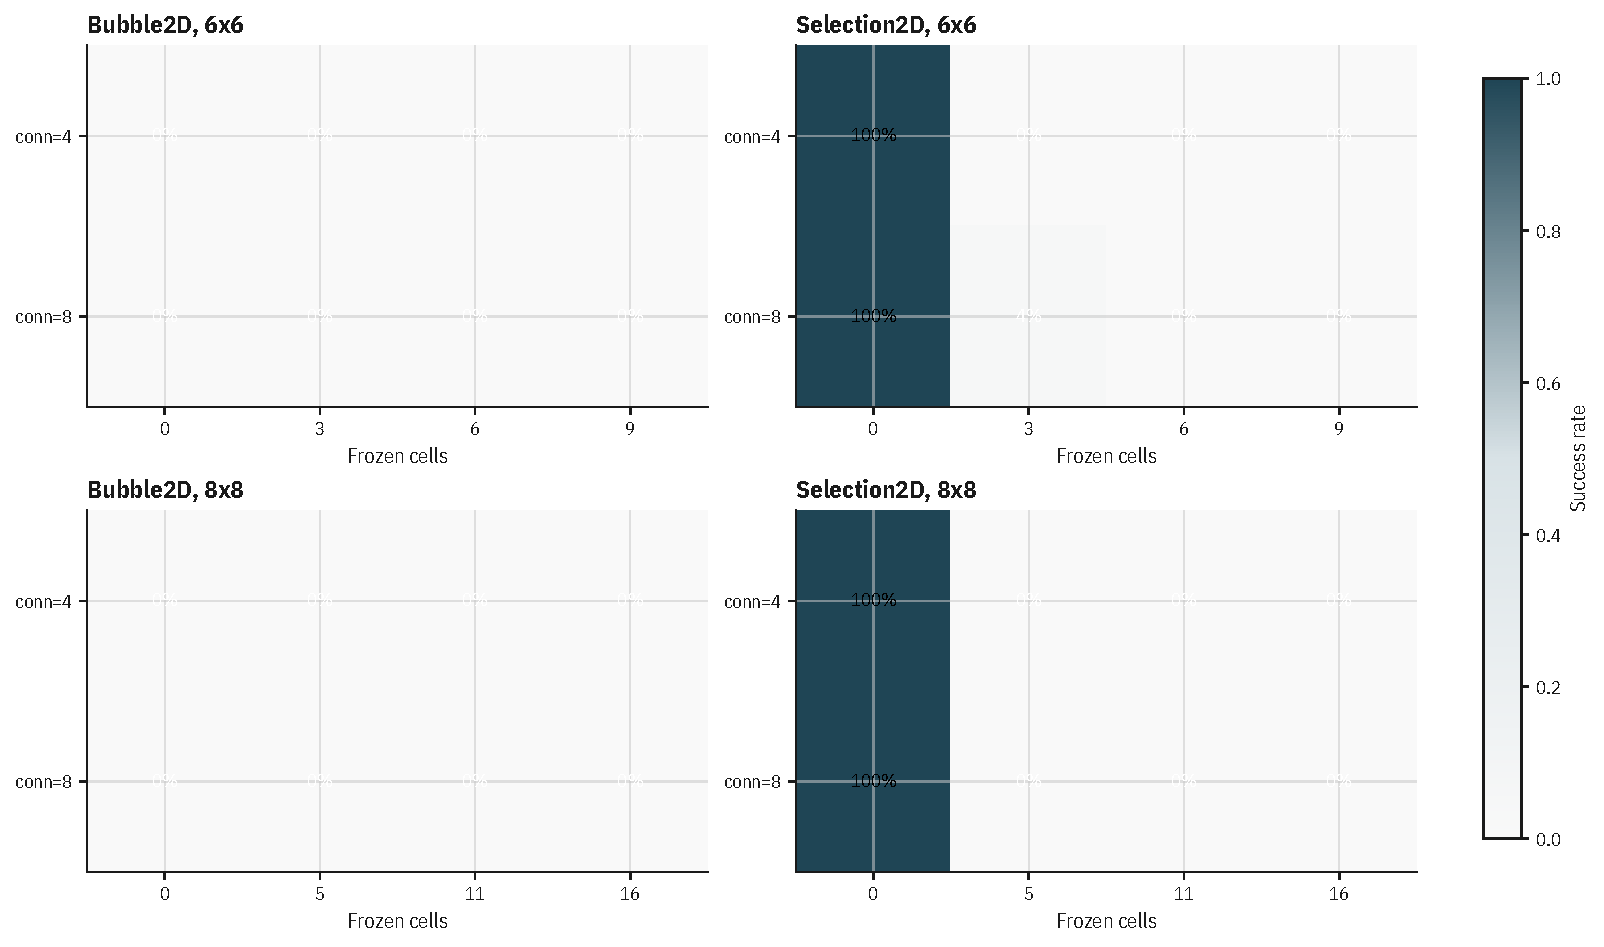
\includegraphics[width=\linewidth]{figures/fig3_2d_success_heatmaps.pdf}
  \caption{\textbf{Canonical 2D success heatmaps (shell ordering).}
  Success rates for Bubble2D and Selection2D across frozen counts and 4/8-connectivity, for grid
  sizes $6\times 6$ and $8\times 8$. Results summarize $100$ trials per configuration, with
  max-steps set to $30\cdot \text{grid\_size}^2$. Even when 8-connectivity expands the local
  neighborhood, purely local algorithms do not reliably escape 2D local minima under this target
  order.}
  \label{fig:2d-heatmaps}
\end{figure}

\subsection{Dip trajectories: delayed gratification}
The paper's ``delayed gratification'' claim is that cells may temporarily worsen a global error
metric to achieve later improvement. We quantify this across $50$ trials per condition.

In 1D with $n=30$ and 3 movable frozen cells, $100\%$ of Bubble runs exhibit at least one dip
(mean $34.2$ dips per trial, mean depth $0.9$ monotonicity errors, mean recovery $2.4$ steps),
while $98\%$ of Selection runs do (mean $3.6$ dips, mean depth $0.4$, mean recovery $0.6$ steps).
In 1D, Bubble is substantially more dip-prone: its local dynamics generate many small oscillations
around movable obstacles, whereas Selection's temporary regressions are rare, shallow, and quickly
resolved. On this metric, 1D dip statistics do not cleanly track goal-directedness; they mostly
capture local thrashing.

In 2D ($6{\times}6$ grid, 3 immovable frozen cells), $100\%$ of Selection2D runs exhibit dips
(mean $308.7$ per trial, mean depth $3.6$ shell inversions, mean recovery $7.2$ steps), while
Bubble2D shows no detected dips. Under this shell-order metric, Bubble2D stalls without producing
recoverable peaks, so the delayed-gratification signature becomes informative only in 2D, where the
goal-directed algorithm generates sustained progress against which temporary setbacks can be
measured.

Figure~\ref{fig:dips} shows representative trajectories; these are fixed-seed exemplars chosen as
the first dip-bearing trial when one exists, otherwise the first trial. They are not restricted to
successful runs and are not cherry-picked outliers.

\begin{figure}[t]
  \centering
  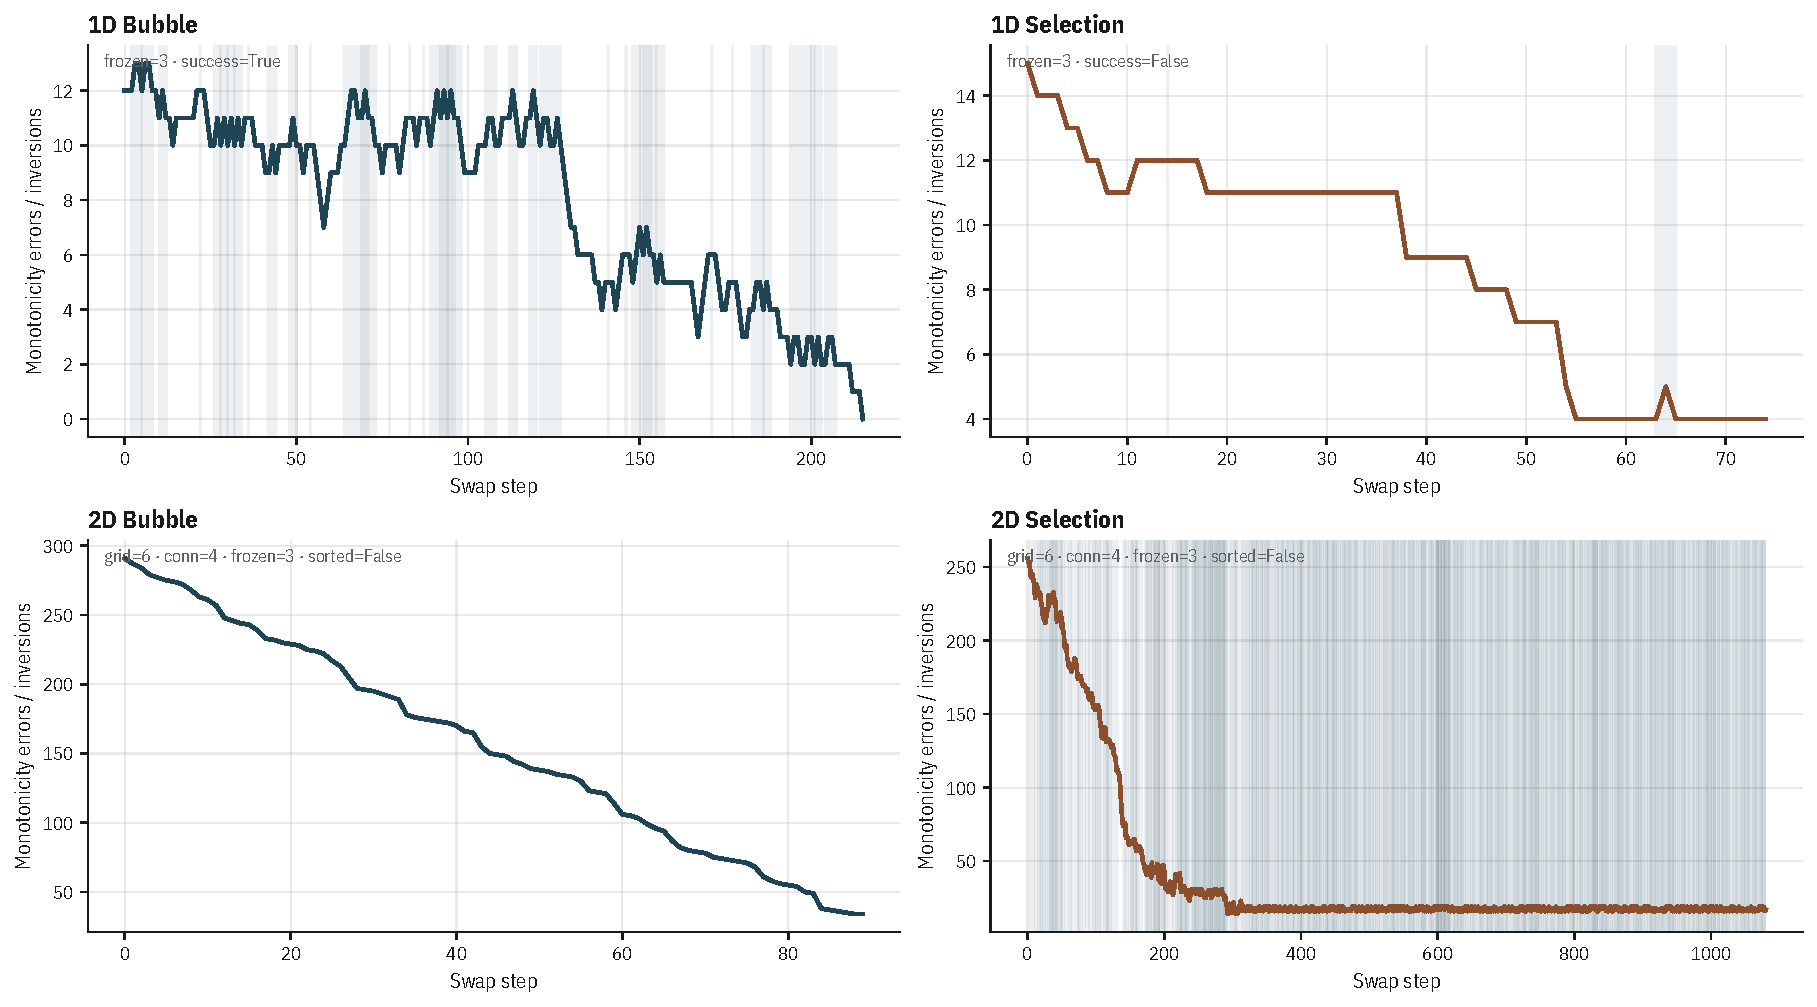
\includegraphics[width=\linewidth]{figures/fig4_dip_trajectories.pdf}
  \caption{\textbf{Dip trajectories (representative).}
  Shaded regions denote detected dip intervals where error temporarily increases and then recovers.
  Top row: 1D monotonicity errors under movable frozen cells. Bottom row: 2D inversion count under
  immovable frozen cells (shell ordering). Aggregate dip statistics across $50$ trials are reported
  in the text.}
  \label{fig:dips}
\end{figure}

\subsection{Topological signature and an algorithm-aligned progress diagnostic}
We apply persistent homology \cite{ghrist2008barcodes} to the swap-interaction graph: nodes are cells and edge weights are
swap frequencies; distances are set as $d = 1/(1+\text{swap\_count})$ and H1 features are computed
via \texttt{ripser} \cite{bauer2021ripser}. In 1D, H1 sharply differentiates Selection from local algorithms; in 2D, H1
counts remain high for both a failing algorithm (Bubble2D: mean $25.6$, success $0\%$) and a
successful one (Selection2D: mean $19.9$, success $100\%$).

This reveals that undirected H1 cycle count conflates local thrashing (Bubble) with directed
goal-seeking (Selection). As a descriptive follow-up, we compute a \emph{Directed Flow} metric: the
ratio of distance-reducing swaps (where the initiating cell moves closer to its ideal position) to
distance-increasing or neutral swaps. For Selection2D this metric is aligned with the same
ideal-position representation used by the policy itself, so we treat it as an algorithm-aligned
diagnostic rather than as independent evidence of competency. On the shell-order $6{\times}6$,
4-neighbor, no-frozen condition used in the right panel of Figure~\ref{fig:h1}, Bubble2D produces
$1835$ forward and $967$ backward initiator swaps across $30$ trials (ratio $1.90$), whereas
Selection2D produces $8741$ forward and $0$ backward initiator swaps. Even with that caveat, the
contrast is useful as a descriptive difference between local thrashing and policy-aligned progress.
Topological complexity alone is not evidence of problem-solving success.

\begin{figure}[t]
  \centering
  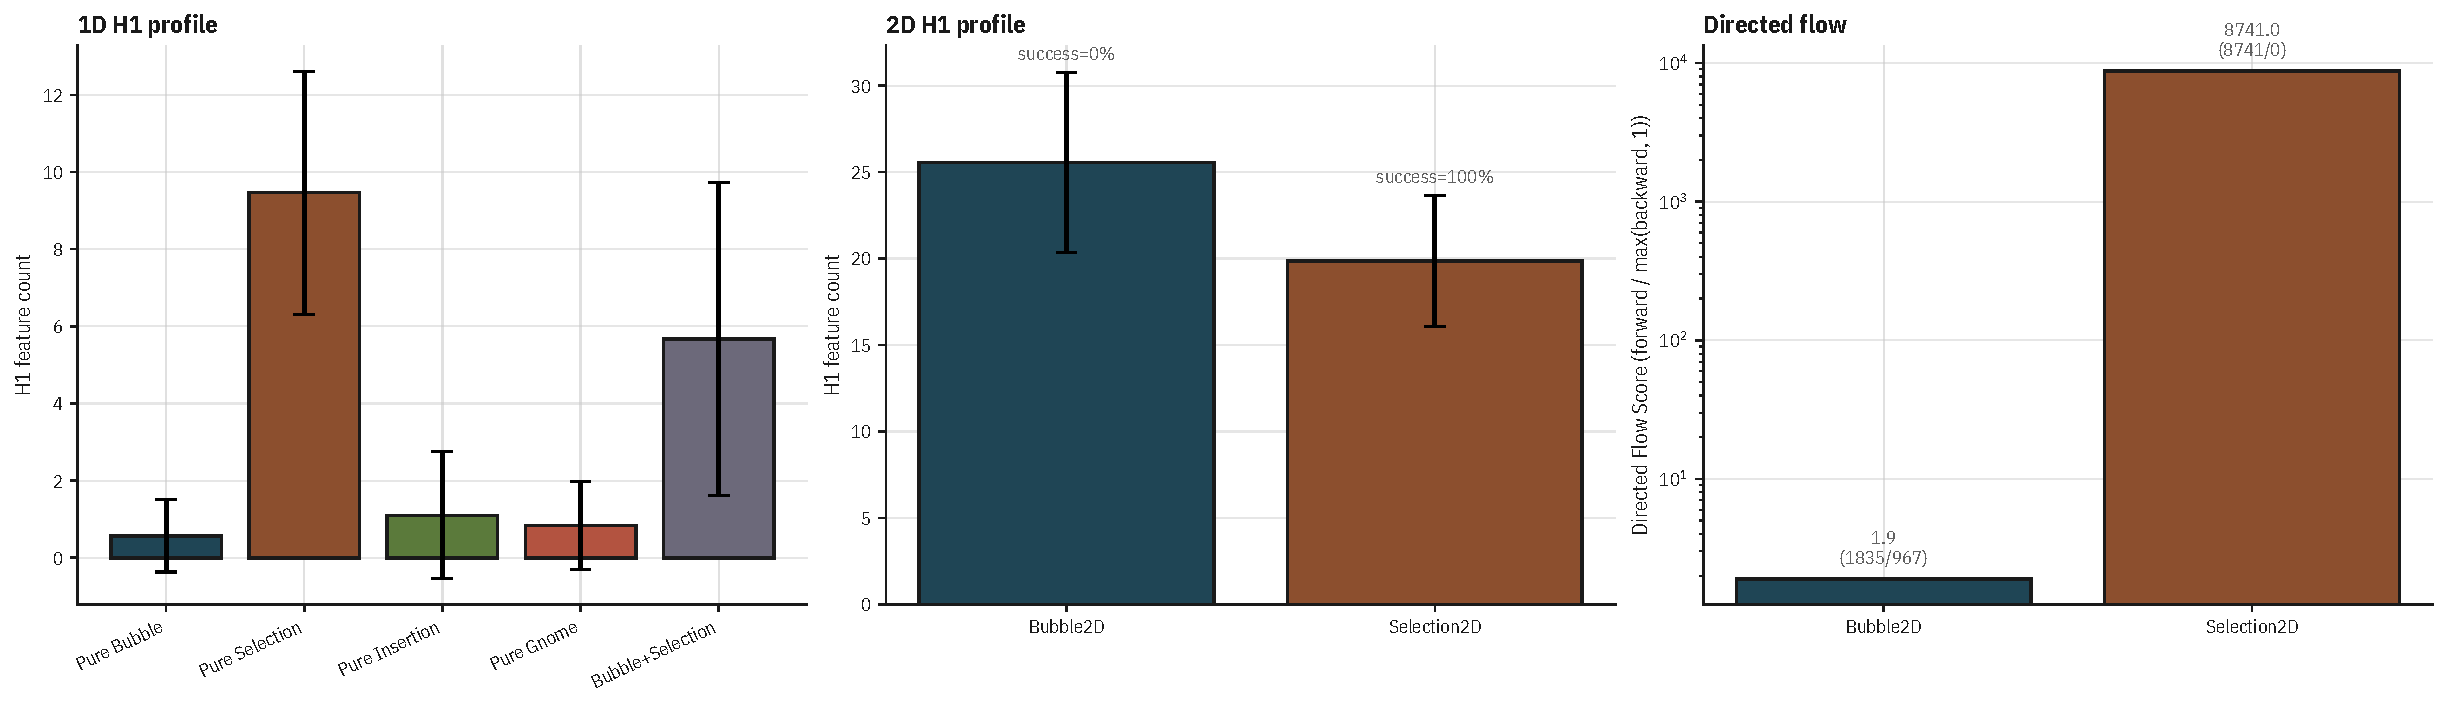
\includegraphics[width=\linewidth]{figures/fig5_h1_bar.pdf}
  \caption{\textbf{H1 features vs.\ Directed Flow.}
  Left/Middle: Undirected H1 separates 1D algorithms but fails to distinguish a failing algorithm (Bubble2D) from a successful one (Selection2D) in 2D. Right: Directed Flow is a useful descriptive diagnostic on the shell-order $6\times 6$, 4-neighbor, no-frozen condition, but because it is defined with respect to each cell's ideal position it should be read as policy-aligned rather than task-neutral. H1 statistics use $30$ trials; Directed Flow uses $30$ trials per 2D condition.}
  \label{fig:h1}
\end{figure}

\section{Matched State-Space Search Efficiency (K-Computation)}
\label{sec:k-computation}
Chis-Ciure and Levin \cite{chisciure2025cognition} operationalize intelligence as search efficiency
in a problem space $\mathcal{P} = \langle S, O, C, E, H \rangle$, where $S$ is the state space,
$O$ the set of operators (with costs), $C$ the constraint set (forbidden state-operator pairs),
$E$ an evaluation functional, and $H$ the effective look-ahead horizon.
The K metric compresses the ratio of blind to guided search cost into a logarithmic scale:
\[
K \;=\; \log_{10}\!\left(\frac{\tau_{\text{blind}}}{\tau_{\text{agent}}}\right),
\]
where $\tau_{\text{blind}}$ is the expected cumulative cost under a maximal-entropy (unbiased)
random walk and $\tau_{\text{agent}}$ is the expected cost under the system's actual policy
\cite{fields2022competency}.
$K = 0$ marks chance; each integer increment corresponds to one order of magnitude of search
advantage.

\paragraph{Problem-space mapping.}
We therefore restrict the metric to the immovable
factorization, where operator classes and frozen-index constraints are explicit and fixed within
each condition. The sorting-cell model then instantiates the formalism as follows:
\begin{itemize}
  \item $S$: the reachable active-value permutations for a fixed frozen-index pattern.
  For long-range Selection, any permutation of the active values is reachable, so
  $|S| = (n_{\text{active}})!$. For adjacent sorting under immovable barriers, only within-segment
  permutations are reachable, so $|S| = \prod_r s_r!$ where $s_r$ are the active segment lengths.
  \item $O$: two matched operator families. The long-range family uses active-active transpositions;
  the adjacent family uses active-active adjacent swaps.
  \item $C$: immovable frozen indices remove state-operator pairs. For the adjacent family, this
  can disconnect the initial state from the goal entirely; for the long-range family, it reduces
  the active state space without eliminating transpositions across frozen barriers.
  \item $E$: active-subsequence sortedness, equivalent to zero inversion count after removing frozen
  indices from the readout.
  \item $H$: the finite factorization-trial horizon.
\end{itemize}

\paragraph{K results.}
Exact maximal-entropy operator-walk hitting times on these $n=30$ state graphs are intractable, so
we make the null explicit at the state-space level. Our blind baseline proposes a reachable state
uniformly at random and pays the matched mean operator cost per proposal, giving
\[
\tau_{\text{blind}}^{\text{state}} \;=\; |S_{\text{reachable}}| \,\bar{w},
\]
where $\bar{w}$ is the mean admissible operator cost under the relevant family and frozen pattern.
For the long-range family we use a distance-weighted transposition cost $w(o)=|i-j|$; for the
adjacent family this reduces to $w(o)=1$. Agent cost uses the realized span-weighted move cost per
attempt, $c = \texttt{total\_move\_distance}/2$, and folds failures into an effective cost-to-first-
success
\[
\tau_{\text{agent}}^{\text{eff}} \;=\; \bar{c}/p_{\text{success}},
\]
computed over reachable trial instances only. If $p_{\text{success}} = 0$, K is undefined.
This null is exact for the stated state-proposal process. If one instead insists on an
operator-walk interpretation, the same quantity is conservative because blind graph traversal can
only increase hitting cost relative to direct random state proposals.

Under this definition, all four Selection-family variants show large positive state-space
K at frozen$=0$: published long-range Selection and its stubborn no-frozen control both achieve
$K_{\text{state}} \approx 30.44$, while the adjacent variants achieve
$K_{\text{state}} \approx 29.80$ and $29.79$. Under immovable frozen indices, the matched long-range
rerouting curve declines monotonically as the reachable state space shrinks from $30!$ to $21!$,
but remains strongly supra-random:
$30.44 \rightarrow 26.14 \rightarrow 22.01 \rightarrow 18.01$ for frozen counts
$0,3,6,9$. By contrast, long-range stubborn Selection has $K_{\text{state}}$ only at frozen$=0$; it
becomes undefined as soon as any frozen indices are introduced because success drops to $0/30$.

The adjacent family exposes a different K-based failure mode. At frozen$=0$, both adjacent variants
have well-defined positive $K_{\text{state}}$, but at frozen $3/6/9$ the adjacent-plus-immovable
problem space is disconnected for every sampled factorization trial: reachable fraction $0/30$ in each
condition. Thus K is undefined there for structural reasons, not merely because the policy is bad.
This is precisely the operator-and-constraint point the previous mixed K surface obscured.

\begin{figure}[t]
  \centering
  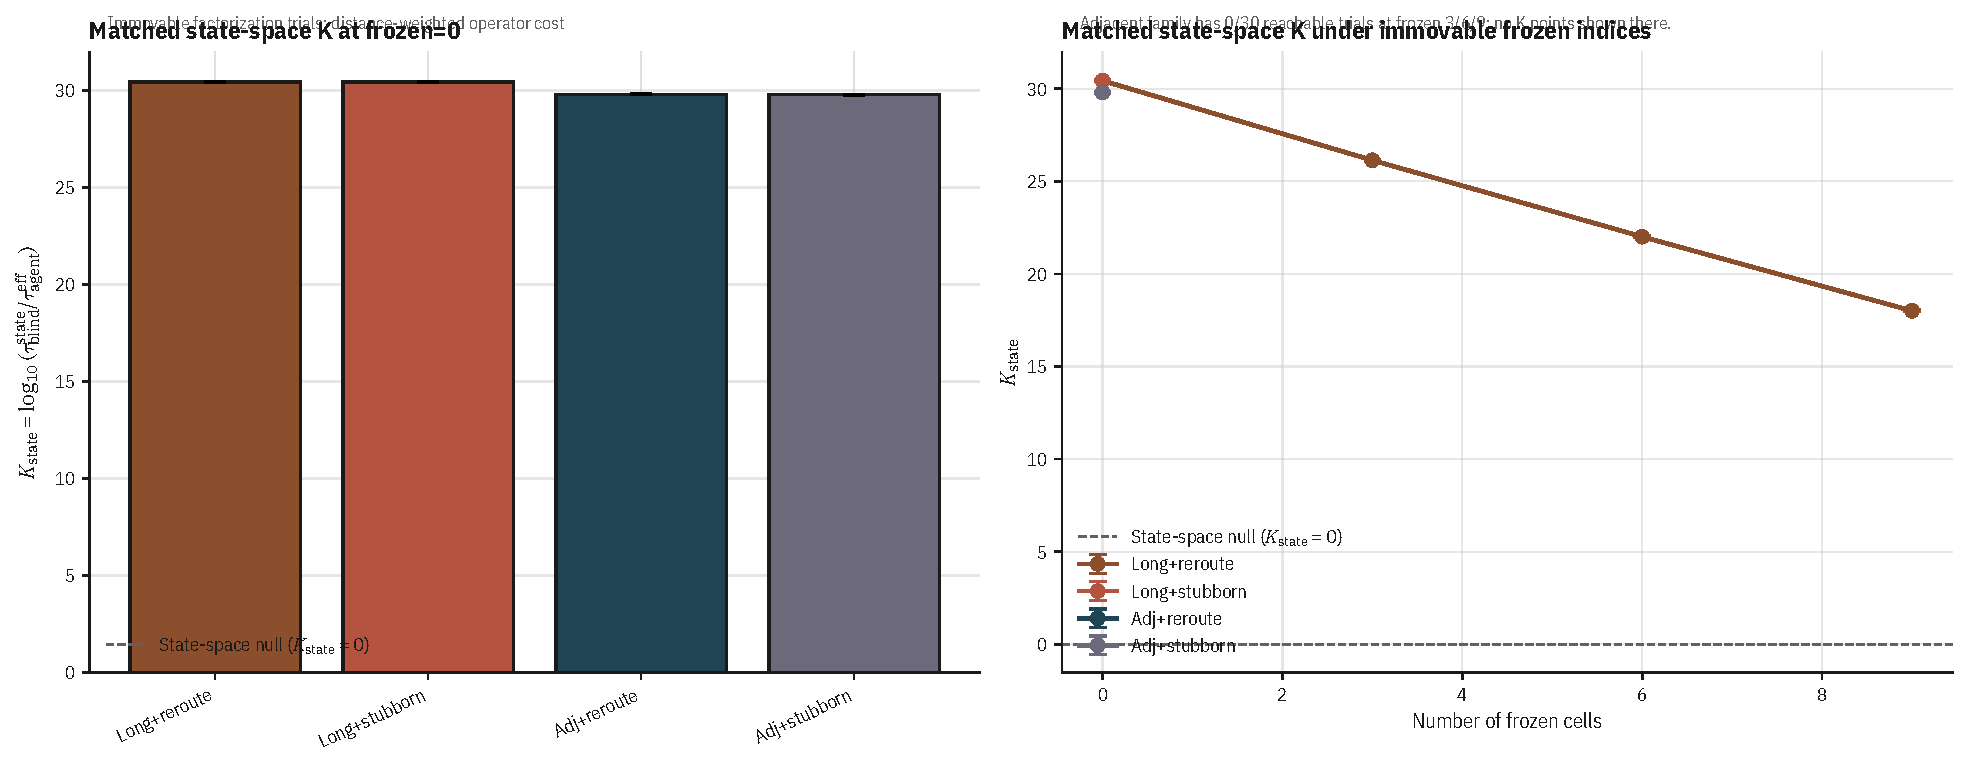
\includegraphics[width=\linewidth]{figures/fig6_k_values.pdf}
  \caption{\textbf{Matched state-space K on the immovable factorization.}
  Left: all four Selection-family variants have large positive exact state-space K at frozen$=0$, but the
  adjacent variants are weaker because they spend more span-weighted work to traverse the same
  reachable state space. Right: when the exact state-space blind baseline is recomputed under each
  frozen pattern, long-range rerouting remains strongly supra-random while declining with the
  active state-space size. Long-range stubborn has undefined K once success drops to zero. The
  adjacent family has no reachable trial instances at frozen $3/6/9$, so no K points appear there.
  Error bars show 95\% bootstrap CIs. The same quantity is also a conservative surrogate for blind
  operator-walk search.}
  \label{fig:k-values}
\end{figure}

\paragraph{Interpretation.}
This K surface is exact for an explicit state-space null and conservative under a stricter
operator-walk reading, while remaining
tied to explicit operator families, explicit frozen constraints, and a distance-weighted cost
model. That is much closer to the formal role K is meant to play in the Diverse Intelligence
framework. Within the long-range operator class, rerouting preserves search efficiency under frozen
barriers; within the adjacent class, the barrier semantics can eliminate reachability altogether.

\section{Discussion}
\label{sec:discussion}
\paragraph{Mechanism-first interpretation.}
Clustering in this model does not require attraction, communication of type, or explicit
coordination. Temporal separation appears to be a major contributor: when one type is active early
and another late, swaps occur in temporally correlated bursts that amplify adjacency among
currently-active types.
This interpretation preserves the morphogenetic analogy but shifts emphasis from ``intelligence'' to
heterochronic dynamics. In developmental biology, heterochrony (shifts in the relative timing of
developmental events) is a primary mechanism for generating morphological diversity
\cite{gould1977ontogeny}. The clustering result instantiates this at a computational level: the
``developmental events'' are sorting phases, and timing shifts between them produce spatial pattern
(clustering) without any explicit patterning instruction. The ablation result (Section~3.2)
strengthens this reading, especially for Insertion-containing mixtures: removing the timing shift
reduces the pattern sharply, just as eliminating a heterochronic gene shift can collapse an evolved
morphological distinction.

\paragraph{Active-matter framing (MIPS).}
The clustering mechanism can be framed as motility-induced phase separation: algorithmic rules define
effective motility profiles, with Selection exhibiting sustained early motion and Insertion remaining
quiescent until its enable-to-move condition is met. Temporal separation then creates regions of
kinematic arrest that accumulate like-typed agents. The InsertionNoWait ablation equalizes motility
profiles and removes clustering, consistent with this interpretation.

\paragraph{Exclusion-process framing (inhomogeneous TASEP).}
The 1D lattice with hard-core exclusion admits a TASEP-style interpretation in which frozen cells and
high-latency algotypes act as transport defects. These defects reduce local flux and induce jammed
phases with upstream density buildup. Under immovable constraints, local algorithms fail in ways
consistent with persistent blockages, while Selection’s non-local target assignment effectively
bypasses local exclusion constraints.

\paragraph{Robustness is semantic and algorithmic.}
Our ablations and matched baselines emphasize a simple point: robustness depends strongly on
operator class, blocked-target policy, and obstacle semantics (movable vs.\ immovable).
The factorization result is the cleanest result here. Under immovable barriers, rerouting alone is
not enough and long-range reach alone is not enough; only the combination survives. The rerouting
ablation then isolates that half of the story within the published long-range Selection operator class. Bubble and
Insertion fail for combinatorial reasons once adjacent transpositions are blocked by hard barriers.
In the same immovable regime, distributed execution does not out-perform centralized baselines
(in the archived centralized comparison).
Zhang et al.\ motivate the cell-view model partly through analogy to basal cognition in living
systems. That centralized-baseline result does not undermine this analogy but sharpens it: whatever
``intelligence'' the sorting cells display comes from the algorithm (the decision rule for when and
how to swap) and is independent of the distributed vs.\ centralized substrate. This is consistent
with Levin's framework \cite{levin2022technological}, which locates competency in the policy (the
mapping from sensory state to action) independent of the particular implementation of that policy.
While multithreaded execution adds strictly computational overhead in an \emph{in-silico} simulation, it remains an essential architectural constraint when modeling physically embodied systems (like biological cells or robotic swarms) where a global ``centralized loop'' is physically impossible.

\paragraph{2D reveals limits of purely local information.}
The 2D shell-ordering target exposes non-adjacent inversions that local neighbor rules cannot resolve
reliably. Selection's explicit ideal position acts as a surrogate for positional information
\cite{wolpert1969positional}, suggesting a computational analogy: any system that must route
components to distant target positions through a constrained grid needs some form of non-local
information. Selection's ideal-position target is a minimal version of this, but it degrades under
frozen cells in 2D (unlike 1D), suggesting that two-dimensional morphogenesis demands richer
guidance signals than a static positional target alone. The section is now reproducible from a
canonical raw-trial archive, but it remains narrower in scope than the 1D factorization and
baseline results.

\paragraph{Search efficiency as a graded metric.}
The K analysis translates the operator-and-constraint story into a graded efficiency metric without
hiding behind a fixed blind
baseline. Because the state-space null is recomputed under each frozen pattern, long-range
Selection's K now falls from $30.44$ to $18.01$ as the reachable state space contracts, rather than
artificially rising under harder conditions. The same framework also clarifies two distinct
failure modes: long-range stubborn Selection retains a reachable problem space but loses all
successful trajectories, whereas the adjacent family under immovable barriers loses reachability in
the sampled factorization instances altogether.
This is the paper's clearest worked state-space proxy for the Diverse Intelligence program's graded
view of competency \cite{levin2022technological,fields2022competency}. It provides a concrete
example of Chis-Ciure and Levin's formalism \cite{chisciure2025cognition} with explicit $O$, $C$,
and $w$. Because the blind numerator is computed under a reachable-state proposal null rather than
an exact maximal-entropy operator walk, we interpret it as an exact $K_{\mathrm{state}}$ analysis
and, secondarily, as a conservative surrogate for blind operator-walk search.

\section{Related Work}
\label{sec:related}

\paragraph{The claims we test.}
Zhang et al.\ \cite{zang2024classical} make three core claims about their sorting-cell model:
that algotype clustering emerges without explicit coordination, that the
distributed cell-view implementation confers robustness akin to ``basal intelligence,'' and that
cells ``navigate'' around damage. In the published implementation, however, those claims sit on top
of specific operator semantics: 1D Selection is not an adjacent-swap rule. Our contribution is to
convert the claims into testable hypotheses and apply causal interventions: ablation of the timing
mechanism (clustering), factorization of action range vs.\ rerouting (navigation), and matched
centralized baselines (cell-view advantage).

\paragraph{Morphogenesis and self-organization.}
Classic accounts of morphogenesis include reaction--diffusion pattern formation
\cite{turing1952chemical} and positional-information frameworks \cite{wolpert1969positional}.
Our temporal-separation result sits closer to the positional-information tradition: clustering
arises not from local chemical gradients but from timing differences between sorting phases,
analogous to heterochrony in developmental biology \cite{gould1977ontogeny}.

On the computational side, local-to-global coordination is central to distributed algorithms
\cite{lynch1996distributed}, swarm intelligence \cite{bonabeau1999swarm,couzin2009collective},
and swarm robotics \cite{rubenstein2014programmable,werfel2014designing}. The sorting-cell model is
distinguished by its extreme minimality: no explicit communication, no shared memory beyond the
array, and no coordination protocol.

\paragraph{Diverse Intelligence and K-computation.}
Levin's ``mind everywhere'' framework treats adaptive, goal-like behaviors as graded phenomena
across substrates \cite{levin2022technological}. Chis-Ciure and Levin \cite{chisciure2025cognition}
formalize this via the K-computation metric, operationalizing intelligence as search efficiency
in a problem space $\mathcal{P} = \langle S, O, C, E, H \rangle$. Our
K analysis provides a worked example of how the abstract formalism maps onto a specific model with
measurable $\tau_{\text{blind}}$ and $\tau_{\text{agent}}$. Fields and Levin
\cite{fields2022competency} develop the broader theoretical context of competency navigation; we
ground their framework in a system small enough that every parameter is inspectable.

\section{Limitations}
\label{sec:limits}
\paragraph{Concurrency and nondeterminism.}
The multithreaded cell-view implementation can exhibit run-to-run variation due to thread scheduling,
even when RNG seeds are fixed. Where this matters, we recommend reporting multi-seed aggregates and
archiving raw run artifacts used to produce figures and tables.

\paragraph{2D scope.}
The 2D archive now regenerates from a single canonical raw-trial pipeline, but the 2D evidence
still covers a narrower slice of the design space than the 1D core: two shell-order algorithms,
two alternate-order controls, and fixed step budgets. We therefore treat the 2D boundary as
reproducible but narrower in scope than the 1D factorization and substrate results. Directed Flow
and related progress diagnostics remain exploratory.

\paragraph{Semantics sensitivity.}
Several headline behaviors depend qualitatively on semantics that are easy to gloss over: whether
frozen elements are movable or immovable, how completion is detected, and which ordering target is
used in 2D. Claims about robustness or ``navigation'' should be interpreted only relative to an
explicitly stated semantics.

\section{Conclusion}
We extend Zhang et al.'s sorting-cell model by isolating mechanisms and making the operator
semantics explicit. The strongest archival result is now a factorization result: under immovable
obstacles, published 1D Selection is robust only when long-range action and frozen-target rerouting
are both present. The rerouting ablation then shows that rerouting is necessary within that
original long-range operator class. Under matched frozen-index semantics, cell-view execution does
not provide an additional robustness advantage over centralized baselines, and the matched-substrate
analysis further shows that changing only the cell-view substrate mostly changes compare-count work
rather than which conditions succeed.
The main explanatory
weight therefore lies in algorithmic rules, operator classes, and obstacle semantics rather than in
distributed execution itself.

Temporal separation has substantially stronger mechanistic support. The original
InsertionNoWait ablation still matters, but the transfer experiment shows that exporting the same waiting gate to
Bubble and Gnome clones reproduces the predicted rise in separation and clustering under matched
same-family controls. We still do not claim a fully closed universal account, but the mechanism
extends beyond one native algotype. The 2D section is regenerated from a canonical raw-trial
archive, but it remains narrower in scope than the 1D core. Directed Flow remains a useful but
policy-aligned exploratory diagnostic. K-computation, by contrast, is framed as a matched
state-space analysis rather than as a descriptive fixed-baseline curve.

The sorting-cell model remains valuable precisely because its components are inspectable. Once the
operator set, obstacle semantics, and baselines are stated explicitly, it becomes a cleaner test bed
for operationalizing graded competence in distributed systems and for separating genuine mechanism
from metaphor in the Diverse Intelligence program.

\appendix

\section{Experiment Semantics and Reproducibility}
\label{sec:appendix-repro}

\subsection{Per-experiment semantics and scale}
\begin{table}[h]
  \centering
  \footnotesize
  \setlength{\tabcolsep}{5pt}
  \renewcommand{\arraystretch}{1.08}
  \begin{tabularx}{\linewidth}{@{}p{0.30\linewidth} p{0.20\linewidth} p{0.14\linewidth} X@{}}
    \toprule
    Experiment surface & Obstacle semantics & Scale & Trials \\
    \midrule
    Pairwise clustering figures & Baseline (no frozen) & $n=30$ / $n=50$ & $50$ (pairwise summary), $20$ (ablation) \\
    Selection factorization & Immovable + movable control & $n=30$ & $10 \times$ 3 seeds (immovable), $5 \times$ 3 seeds (movable) \\
    Frozen-target rerouting ablation & Immovable & $n=30$ & $30 \times$ 3 seeds \\
    Centralized baseline comparison & Immovable & $n=30$ & $12 \times$ 3 seeds \\
    Matched substrate comparison & Immovable & $n=30$ & $3 \times$ 3 seeds (original trio), $3 \times$ 3 seeds (Selection family) \\
    Canonical 2D heatmaps & Immovable & $6{\times}6$, $8{\times}8$ & $100$ per configuration \\
    Dip exemplars & Movable (1D), immovable (2D) & $n=30$, $6{\times}6$ & Single exemplars; $50$ aggregate trials \\
    H1 / Directed Flow & Baseline (no frozen) & $n=30$, $6{\times}6$ & $30$ per condition \\
    Matched state-space K & Immovable & $n=30$ & Derived from factorization raw trials \\
    \bottomrule
  \end{tabularx}
  \caption{Per-experiment obstacle semantics, scale, and archive size. The repository keeps numeric script ids, but the main text refers to these surfaces descriptively.}
  \label{tab:semantics}
\end{table}

\subsection{Command index}
All experiments live in \texttt{dossiers/zang-levin-playground/}. The repository keeps numeric
script ids for archival continuity; the main text refers to the same surfaces descriptively.

\paragraph{Clustering and timing.}
\begin{itemize}
  \item Pairwise temporal separation vs.\ clustering:
  \begin{quote}\small
  \texttt{\detokenize{uv run python paper/compute_fig1_temporal_clustering.py}}
  \end{quote}
  \item Clustering ablation:
  \begin{quote}\small
  \texttt{\detokenize{uv run python paper/run_clustering_ablation.py}}
  \end{quote}
  \item Synthetic timing-gate transfer:
  \begin{quote}\small
  \texttt{\detokenize{for s in 40 41 42; do}}\\
  \texttt{\detokenize{  uv run python exp27_timing_interventions.py}}\\
  \texttt{\detokenize{    --base-seed $s --n-trials 10}}\\
  \texttt{\detokenize{    --out paper/results/exp27_seed${s}_n50_t10.json;}}\\
  \texttt{\detokenize{done}}
  \end{quote}
  Aggregate with:
  \begin{quote}\small
  \texttt{\detokenize{uv run python paper/aggregate_exp27_timing_interventions.py --inputs ...}}
  \end{quote}
\end{itemize}

\paragraph{1D robustness and substrate comparisons.}
\begin{itemize}
  \item Selection factorization, immovable:
  \begin{quote}\small
  \texttt{\detokenize{for s in 40 41 42; do}}\\
  \texttt{\detokenize{  uv run python exp25_selection_factorization.py}}\\
  \texttt{\detokenize{    --seed $s --n-trials 10 --timeout 5 --semantics immovable}}\\
  \texttt{\detokenize{    --out paper/results/exp25_seed${s}_n30_t5_immovable.json;}}\\
  \texttt{\detokenize{done}}
  \end{quote}
  \item Selection factorization, movable control:
  \begin{quote}\small
  \texttt{\detokenize{for s in 40 41 42; do}}\\
  \texttt{\detokenize{  uv run python exp25_selection_factorization.py}}\\
  \texttt{\detokenize{    --seed $s --n-trials 5 --timeout 5 --semantics movable}}\\
  \texttt{\detokenize{    --out paper/results/exp25_seed${s}_n30_t5_movable.json;}}\\
  \texttt{\detokenize{done}}
  \end{quote}
  Aggregate with:
  \begin{quote}\small
  \texttt{\detokenize{uv run python paper/aggregate_exp25_selection_factorization.py --inputs ...}}
  \end{quote}
  \item Frozen-target rerouting ablation:
  \begin{quote}\small
  \texttt{\detokenize{for s in 40 41 42; do}}\\
  \texttt{\detokenize{  uv run python exp10_ablation_goal_adjustment.py}}\\
  \texttt{\detokenize{    --seed $s --n-trials 30 --timeout 10}}\\
  \texttt{\detokenize{    --out paper/results/exp10_seed${s}_n30_t10.json;}}\\
  \texttt{\detokenize{done}}
  \end{quote}
  \item Centralized baseline comparison:
  \begin{quote}\small
  \texttt{\detokenize{for s in 40 41 42; do}}\\
  \texttt{\detokenize{  uv run python exp14_cellview_vs_traditional.py}}\\
  \texttt{\detokenize{    --seed $s --n-trials 12 --timeout 10}}\\
  \texttt{\detokenize{    --out paper/results/exp14_seed${s}_n12_t10.json;}}\\
  \texttt{\detokenize{done}}
  \end{quote}
  \item Matched substrate comparison, original trio:
  \begin{quote}\small
  \texttt{\detokenize{for s in 40 41 42; do}}\\
  \texttt{\detokenize{  uv run python exp26_substrate_matched_baselines.py}}\\
  \texttt{\detokenize{    --seed $s --n-trials 3 --timeout 5}}\\
  \texttt{\detokenize{    --max-compare-and-swap 200000}}\\
  \texttt{\detokenize{    --frozen-counts 1,3 --algorithms Bubble,Insertion,Selection}}\\
  \texttt{\detokenize{    --out paper/results/}}\\
  \texttt{\detokenize{      exp26_original_trio_seed${s}_n30_t3_frozen1_3_budget200k.json;}}\\
  \texttt{\detokenize{done}}
  \end{quote}
  \item Matched substrate comparison, Selection family:
  \begin{quote}\small
  \texttt{\detokenize{for s in 40 41 42; do}}\\
  \texttt{\detokenize{  uv run python exp26_substrate_matched_baselines.py}}\\
  \texttt{\detokenize{    --seed $s --n-trials 3 --timeout 5}}\\
  \texttt{\detokenize{    --max-compare-and-swap 200000}}\\
  \texttt{\detokenize{    --frozen-counts 0,1,3,6,9}}\\
  \texttt{\detokenize{    --algorithms Selection,StubbornSelection,}}\\
  \texttt{\detokenize{      AdjacentSelection,AdjacentStubbornSelection}}\\
  \texttt{\detokenize{    --out paper/results/}}\\
  \texttt{\detokenize{      exp26_selection_family_seed${s}_n30_t3_budget200k.json;}}\\
  \texttt{\detokenize{done}}
  \end{quote}
  Aggregate either matched-substrate panel with:
  \begin{quote}\small
  \texttt{\detokenize{uv run python paper/aggregate_exp26_substrate_matched_baselines.py}}\\
  \texttt{\detokenize{  --inputs ...}}
  \end{quote}
\end{itemize}

\paragraph{2D, diagnostics, and figure generation.}
\begin{itemize}
  \item Canonical 2D archive and aggregation:
  \begin{quote}\small
  \texttt{\detokenize{uv run python exp28_2d_canonical.py}}\\
  \texttt{\detokenize{  --out paper/results/exp28_2d_canonical_trials.json}}\\
  \texttt{\detokenize{uv run python paper/aggregate_fig3_2d.py}}\\
  \texttt{\detokenize{  --input paper/results/exp28_2d_canonical_trials.json}}\\
  \texttt{\detokenize{  --heatmap-out paper/results/fig3_2d_success_heatmaps.json}}\\
  \texttt{\detokenize{  --alt-out paper/results/fig3b_alt_orderings.json}}
  \end{quote}
  \item Matched state-space K:
  \begin{quote}\small
  \texttt{\detokenize{uv run python paper/compute_k.py}}
  \end{quote}
  \item H1 summary:
  \begin{quote}\small
  \texttt{\detokenize{uv run python paper/compute_fig5_h1.py}}
  \end{quote}
  \item Directed Flow:
  \begin{quote}\small
  \texttt{\detokenize{uv run python paper/compute_directed_flow.py}}
  \end{quote}
  \item Dip statistics:
  \begin{quote}\small
  \texttt{\detokenize{uv run python paper/compute_dip_stats.py}}
  \end{quote}
  \item Figure generation:
  \begin{quote}\small
  \texttt{\detokenize{uv run python paper/make_figures.py}}
  \end{quote}
\end{itemize}

Thread scheduling introduces nondeterminism even with fixed RNG seeds. We therefore archive JSON
outputs for the paper and report multi-seed aggregates for central claims.

\bibliographystyle{unsrt}
\bibliography{references}

\end{document}
